\documentclass[14pt, a4paper]{report}
\usepackage{mathtext}
\usepackage[T2A]{fontenc}
\usepackage[utf8]{inputenc}
\usepackage[russian]{babel}
\usepackage{multirow}
\usepackage{slashbox}
\usepackage{makecell}
\usepackage{graphicx}
\usepackage{physics}
\usepackage{amstext}
\usepackage{caption}
\usepackage{subcaption}
\usepackage{cmap}
\usepackage{float}
\usepackage{indentfirst}
\usepackage{romannum}

\usepackage[a4paper,
            		left=1in,
            		right=1in,
           		 top=1in,
            		bottom=1in,
            		footskip=.25in]{geometry}

\renewcommand{\thesection}{\arabic{section}.}
\renewcommand{\thesubsection}{\arabic{section}.\arabic{subsection}.}

\title{\textbf{Отчет о выполнении лабораторной работы 1.2 "Исследование эффекта Комптона"}}
\author{Калашников Михаил, Б03-202}
\date{}

\begin{document}
\maketitle

\pagenumbering{arabic}

\textbf{Цель работы:} Исследование энергетического спектра $\gamma$-квантов, рассеянных на графите, с помощью стинцилляционного спектромета. Определение энергии рассеянный $\gamma$-квантов в зависимости от угла рассеяния, а также энергии покоя частиц, на которых происходит комптоновское рассеяние.
\newline

\section{Теоретические сведения}

Рассмотрим элементарную теорию эффекта Комптона. Пусть на покоящийся электрон налетает $\gamma$-квант. После соударения электрон приобретает импульс, а $\gamma$-квант рассеивается на некоторый угол, по отношению к начальному направлению движения. Энергия и импульс $\gamma$-кванта также претерпят изменения. Решая систему уравнений законов сохранения энергии и импульса, получим:

\[\Delta\lambda=\frac{h}{mc}(1-\cos{\theta})\]

Основной целью лабораторной работы является проверка данного соотношения.

\section{Экспериментальная установка}

Блок схема установки изображена на рисунке ниже. Источником излучения служит $^{137}Cs$. Сформированный коллиматором узкий пучок $\gamma$-квантов попадает на графитовую мишень. Кванты, испытавшие комптоновское рассеяние в мишени, регистируются сцинтилляционным счетчиком.

\begin{figure}[H]
\centering
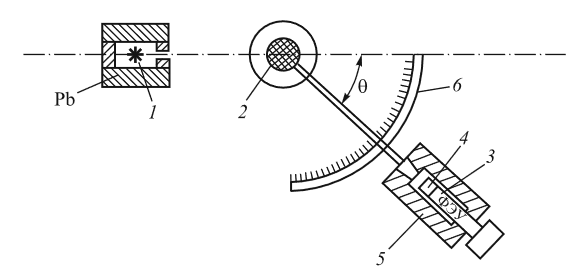
\includegraphics[scale=0.8]{../images/512-1}
\caption{Блок схема установки по изучению рассеяния $\gamma$-квантов}
\end{figure}

\section{Проведение эксперимента}

\section{Обработка результатов}

\section{Выводы}

\end{document}